\section{Gaussian Obstacles}
\subsection{Shape of the Path}
The step-avoiding route shown in Figure 2 is only one example among a family of routes with equal cost. The frequently-employed two-dimensional Gaussian distribution 
%A smoothly-varying obstacle 
breaks this degeneracy and determines a finite number of optimal paths.

%By smoothly-varying, we mean that the derivative of $f$ is defined everywhere. One such example, commonly used to model obstacles, is the Gaussian.

\begin{equation}
f(x, y) = A \exp\left(-\displaystyle\frac{x^2+y^2}{2\sigma^2}\right)
\end{equation}

The Gaussian is radially symmetric, and it decreases monotonically from its center. These properties are reasonable as they ensure that areas closer to the center of the obstacle have higher costs. Due to the symmetry, there will be two equal optimal paths on each side of the $x$-axis. For every optimal path with positive $y$ coordinates, there is an equally optimal negative coordinate one. With that in mind, for purposes of this discussion we shall only consider the non-negative paths. 

One key feature of functions like this that are decreasing monotonically is that the optimal path is always bracket-shaped: from $(-n,0)$ to $(-n, \yhat)$ to $(n, \yhat)$ to $(n,0)$ for some $\yhat$. An example can be seen in Figure \ref{fig:bracket}. Note that a direct path qualifies as a bracket with $\yhat=0$.

We can prove that the optimal path is bracket-shaped. It is easy enough to see that an optimal path would lie only on one side of the $x$-axis (or on it) and would not double back on itself. However that still leaves us with paths like the suboptimal one shown in Figure \ref{fig:bracket}. Let us assume that this other path $p_0$ is optimal. There must be a value $\yhat$ that is the maximum $y$ value attained by the path. We can create another path $p_1$ that has the same length as $p_0$ where each horizontally moving segment is moved up to $\yhat$ and every vertical moving segment is moved to either $-n$ or $+n$ (depending on which side of the $x$-axis it is on). Since $f$ is monotonically decreasing, $p_1$ will have a smaller cost than $p_0$, but since this is impossible (we assumed $p_0$ was optimal, we can conclude that the bracket shape is optimal.  

For the step obstacle in the previous section, the best path was determined by relative size $h/w$ and relative cost $A/P$. We might have predicted as much from dimensional analysis. In the current case, we seek a relationship between these model parameters and $\yhat$, the distance of closest approach.

\begin{figure}
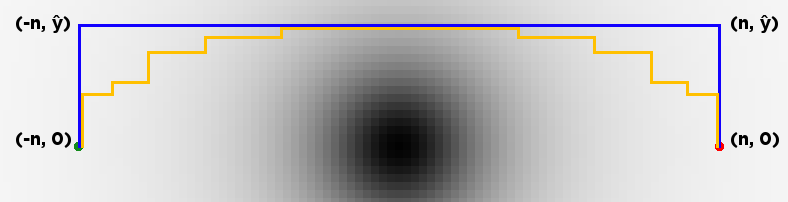
\includegraphics[width=\columnwidth]{graphix/bracket.png}
\caption{The Bracket Shape - The optimal path is shown in blue with the corresponding coordinates. A suboptimal path is shown below it in yellow. }
\label{fig:bracket}
\end{figure}
